\chapter{PENGUJIAN DAN ANALISIS}
\label{chap:pengujiananalisis}

Pada penelitian ini, dipaparkan hasil pengujian serta analisis dari desain sistem dan implementasi. Data yang digunakan dalam pengujian data diambil dari sebagian data yang dipisahkan dari dataset Kaggle \cite{cit:kaggledata}, Webcam \cite{cit:wb500}, dan kamera DSLR \cite{cit:100d}.  Pengambilan data video dilakukan di kompleks perkuliahan departemen Teknik Elektro FTEIC-ITS, dan tempat tinggal penulis. Pengujian dilakukan dalam beberapa bagian sebagai berikut

\section{Skenario Pengujian}
\label{sec:skenariopengujian}

Pengujian dilakukan dengan menjalankan program klasifikasi menggunakan model yang sudah di training menggunakan dataset yang sudah dijelaskan pada bagian \ref{sec:pengumpulandata} untuk mengklasifikasikan gerakan cuci tangan yang berbeda beda dalam satu video. Pengujian yang akan dilakukan diantaranya:
\begin{enumerate}
	\item \textbf{Pengujian Sistem}

	Pada Pengujian Sistem, \textit{Model} yang sudah di training akan diuji dengan melihat hasil \textit{Training History}, \textit{confusion matrix}, dan \textit{Classification Report} menggunakan test dataset yang dibagi oleh \textit{train\_test\_split} yang dijelaskan pada bagian \ref{subsec:traintestsplit}.
	
	Dengan melihat hasil dari pengujian tersebut, kita dapat mengetahui sejauh mana tingkat akurasi model terhadap \textit{Test Set} yang merupakan data yang paling serupa dengan \textit{Training Set}
	
	\item \textbf{Pengujian berdasarkan sudut pengambilan video}

	Pada pengujian ini. sistem diuji tingkat akurasinya terhadap video yang berisikan urutan gerakan cuci tangan yang serupa dengan dataset namun diambil dari sudut yang berbeda dari yang ditetapkan pada dataset training. Akurasi dari pengujian ini dihitung dengan melihat berapa banyak gerakan yang berhasil di klasifikasikan. Pada pengujian ini, diatur \textit{window size} pada moving average sebesar 60 (2 x FPS Video Input)
	
	Di Pengujian ini, digunakan video yang diambil di waktu yang sama saat pengumpulan dataset DSLR, akan tetapi sudut pengambilan / posisi kamera digeser sekitar 40 derajat dari posisi awal, seperti yang dapat dilihat pada gambar
	
	\begin{figure}[!ht]
		\centering
		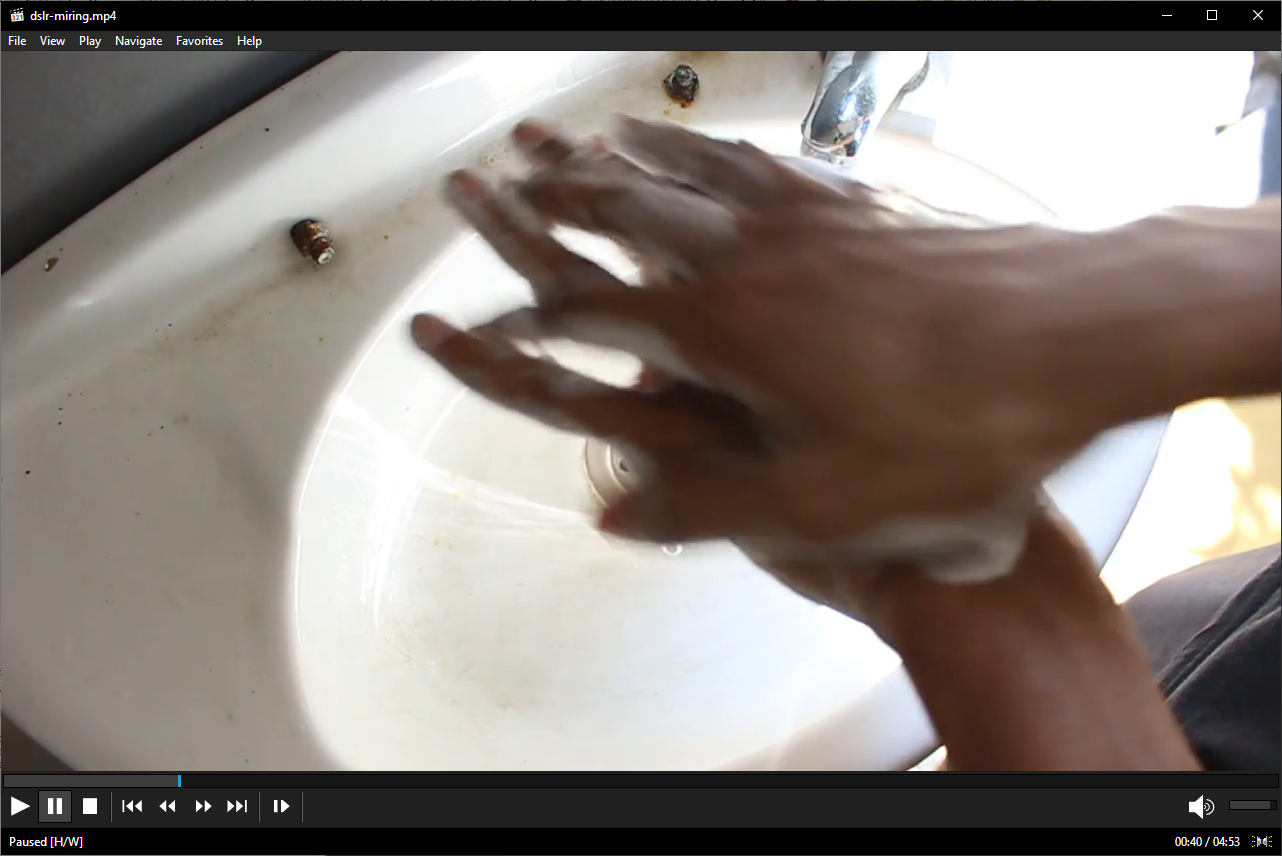
\includegraphics[width=0.6\columnwidth]{gambar/contohsudut.png}
		\caption{Sample sudut pengambilan citra video}
		\label{fig:contohsudut}
	\end{figure}
	
	Dengan melihat hasil dari pengujian tersebut, kita dapat mengetahui bagaimana pengaruh sudut pengambilan gambar terhadap sistem Klasifikasi Gerakan Mencuci Tangan langsung dari output video yang dihasilkan
	
	\item \textbf{Pengujian berdasarkan setup pengambilan video}
	
	Pada pengujian ini. sistem diuji tingkat akurasinya terhadap video yang berisikan urutan gerakan cuci tangan yang diambil dari setup pengambilan video yang berbeda dari dataset. Akurasi dari pengujian ini dihitung dengan melihat berapa banyak gerakan yang berhasil di klasifikasikan. Pada pengujian ini, diatur \textit{window size} pada moving average sebesar 60 (2 x FPS Video Input)
	
	Di Pengujian ini, digunakan video yang diambil menggunakan webcam yang ditempatkan diatas stand setinggi 50cm. webcam diarahkan ke tanah area \textit{wudhu} di tempat tinggal penulis sebagai background nya
	
	\begin{figure}[!ht]
		\centering
		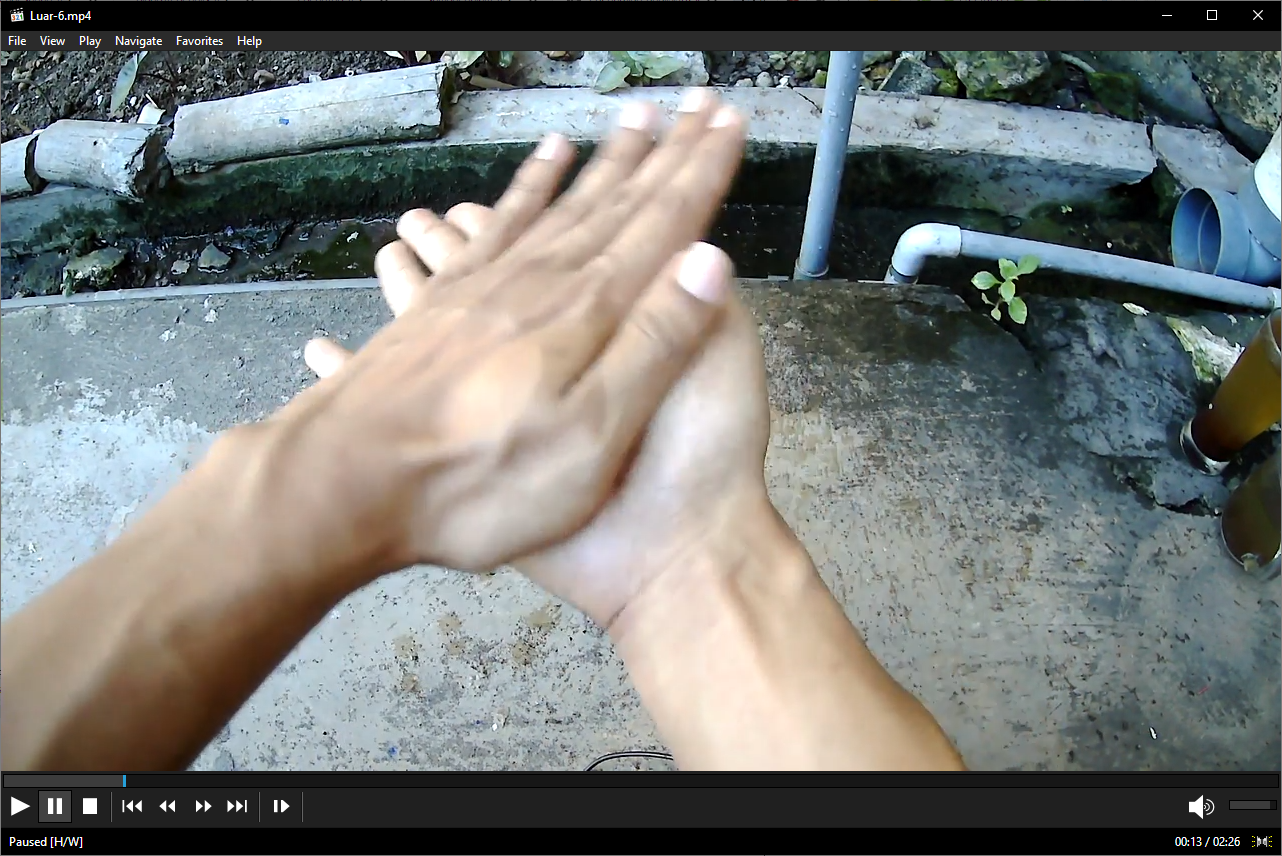
\includegraphics[width=0.6\columnwidth]{gambar/setupwudhu.png}
		\caption{Sample setup pengambilan citra video}
		\label{setupwudhu}
	\end{figure}
	
	Dengan melihat hasil dari pengujian tersebut, kita dapat mengetahui kemampuan generalisasi sistem untuk mengklasifikasikan gerakan cuci tangan dengan setup berbeda langsung dari output video yang dihasilkan
\end{enumerate}

\newpage
\section{Evaluasi Pengujian}
\label{sec:analisispengujian}

Dari pengujian yang dilakukan, dapat diketahui sejauh mana kemampuan sistem yang sudah dibuat dan apa saja batasannya serta bagaimana sistem ini dapat disempurnakan lebih lanjut.

\subsection{Pengujian Sistem}
\label{subsec:ujisistem}

Dari Pengujian yang dilakukan, didapat data sebagai berikut:
\begin{figure}[!ht]
	\centering
	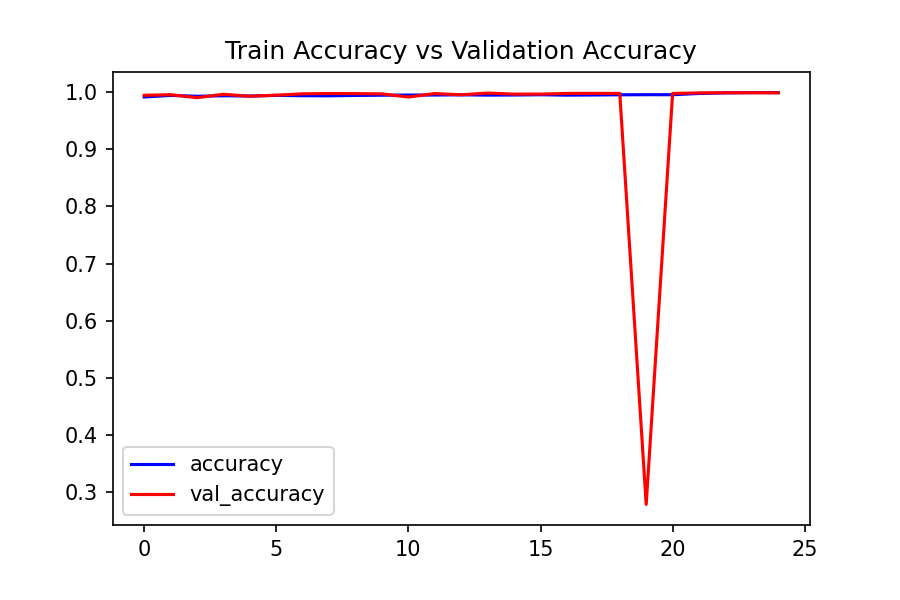
\includegraphics[width=0.5\columnwidth]{gambar/train-val-acc.png}
	\caption{Train and Validation Accuracy}
	\label{fig:train-val-acc}
\end{figure}
\begin{figure}[!ht]
	\centering
	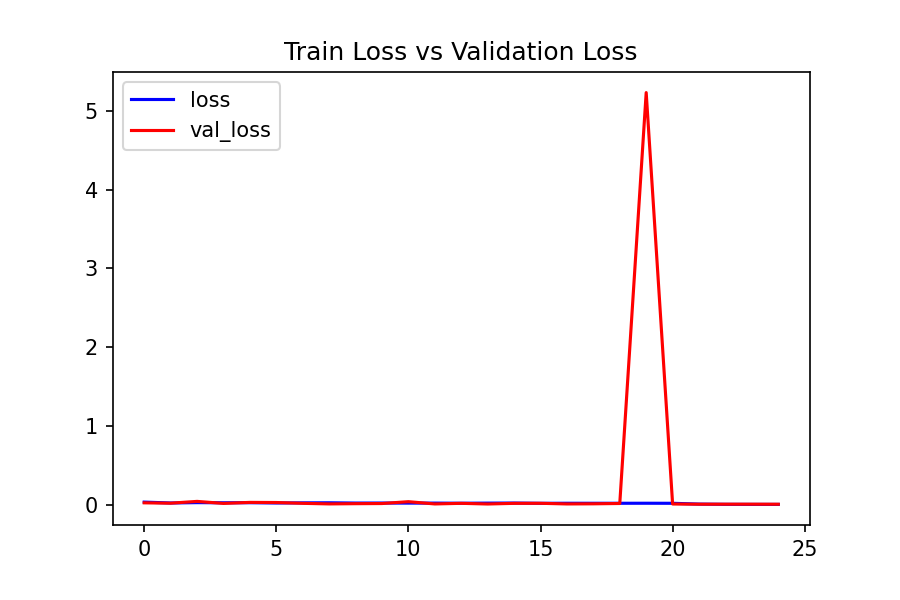
\includegraphics[width=0.5\columnwidth]{gambar/train-val-loss.png}
	\caption{Train and Validation Loss}
	\label{fig:train-val-loss}
\end{figure}

Pada training history, terlihat bahwa Val\_Accuracy dan Val\_loss memiliki spike pada epoch ke 16 hingga 20

\begin{figure}[!ht]
	\centering
	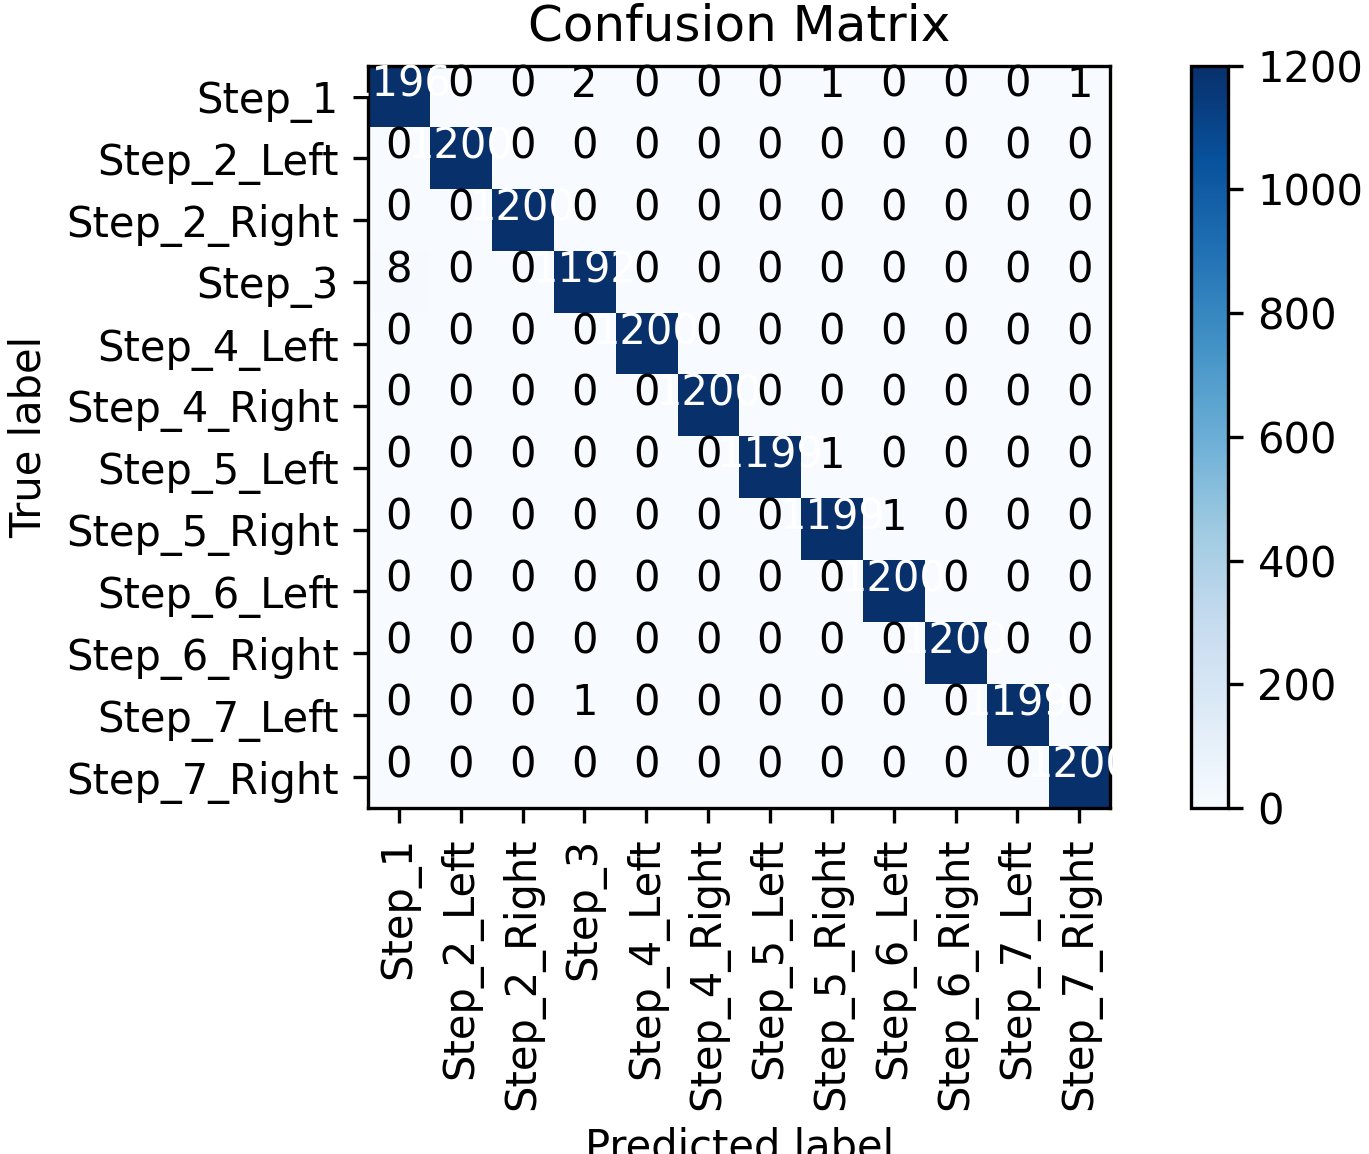
\includegraphics[width=0.6\columnwidth]{gambar/confusion-matrix.png}
	\caption{Confusion Matrix}
	\label{fig:confmatx}
\end{figure}

Berdasarkan Confusion Matrix tersebut, dapat dilihat bahwa model memiliki akurasi yang cukup baik pada test set. hanya sedikit kesalahan yang terjadi terutama pada step\_3 yang memang memiliki citra yang hampir mirip dengan step\_1 yang mana perbedaannya hanyalah terletak pada kondisi jari yang saling bersilangan.

\begin{table}[!ht]
	\centering
	\resizebox{0.5\textwidth}{!}{%
		\begin{tabular}{|l|l|l|l|l|}
			\hline
			& precision   & recall  & f1-score & support \\ \hline
			Step\_1        & 0.99        & 1.00    & 1.00     & 1200    \\ \hline
			Step\_2\_Left  & 1.00        & 1.00    & 1.00     & 1200    \\ \hline
			Step\_2\_Right & 1.00        & 1.00    & 1.00     & 1200    \\ \hline
			Step\_3        & 1.00        & 0.99    & 1.00     & 1200    \\ \hline
			Step\_4\_Left  & 1.00        & 1.00    & 1.00     & 1200    \\ \hline
			Step\_4\_Right & 1.00        & 1.00    & 1.00     & 1200    \\ \hline
			Step\_5\_Left  & 1.00        & 1.00    & 1.00     & 1200    \\ \hline
			Step\_5\_Right & 1.00        & 1.00    & 1.00     & 1200    \\ \hline
			Step\_6\_Left  & 1.00        & 1.00    & 1.00     & 1200    \\ \hline
			Step\_6\_Right & 1.00        & 1.00    & 1.00     & 1200    \\ \hline
			Step\_7\_Left  & 1.00        & 1.00    & 1.00     & 1200    \\ \hline
			Step\_7\_Right & 1.00        & 1.00    & 1.00     & 1200    \\ \hline
			accuracy       & \multicolumn{2}{l|}{} & 1.00     & 14400   \\ \hline
			macro avg      & 1.00        & 1.00    & 1.00     & 14400   \\ \hline
			weighted avg   & 1.00        & 1.00    & 1.00     & 14400   \\ \hline
		\end{tabular}%
	}
	\caption{sklearn Classification Report}
	\label{tab:clasreport}
\end{table}

\subsection{Hasil pengujian berdasarkan Sudut Pengambilan Citra Video}
\label{subsec:ujisudut}

Sample hasil pengujian berdasarkan sudut pengambilan citra video dapat dilihat pada gambar \ref{fig:sudutbenar1} dan \ref{fig:sudutsalah1}

\begin{figure}[!ht]
	\centering
	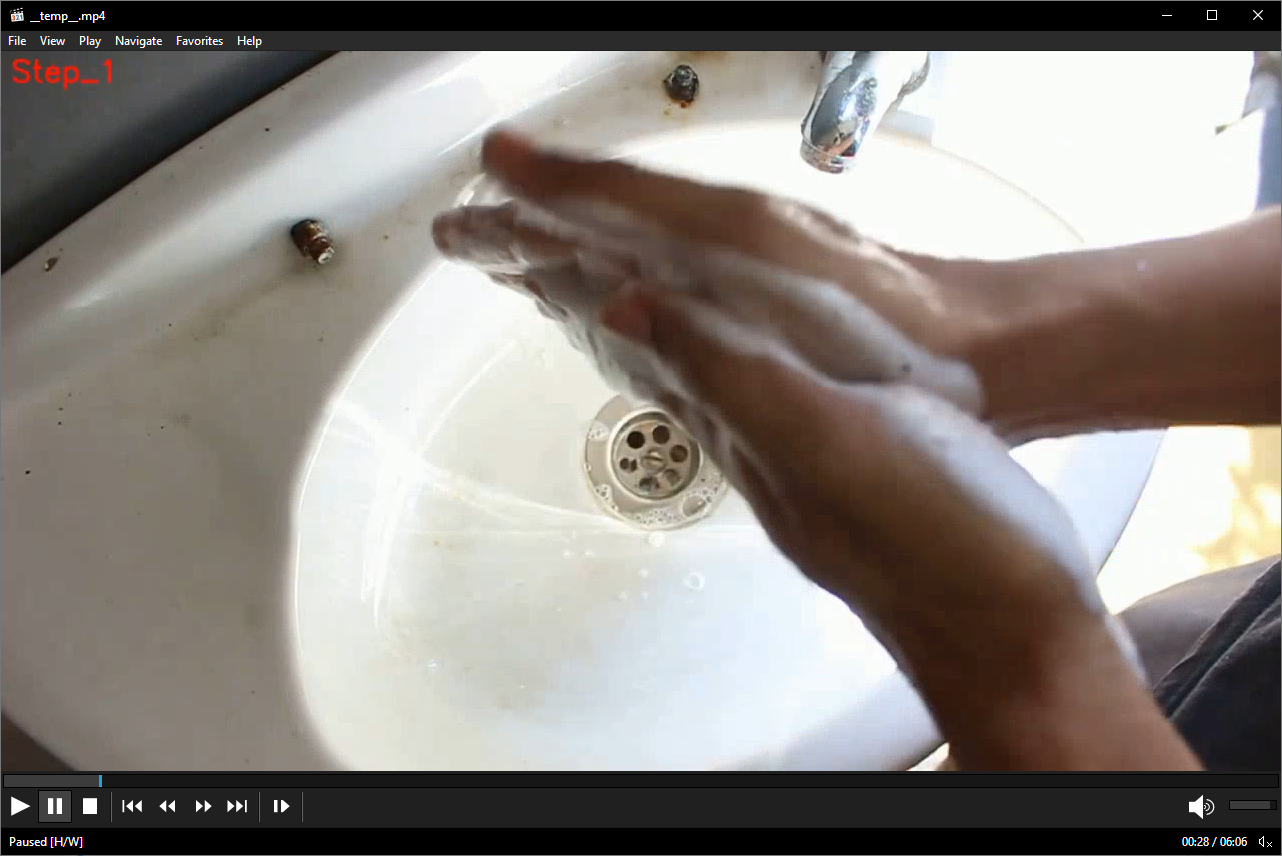
\includegraphics[width=0.6\columnwidth]{gambar/sudutbenar1.png}
	\caption{Pengujian Berdasarkan Sudut (Benar)}
	\label{fig:sudutbenar1}
\end{figure}
\begin{figure}[!ht]
	\centering
	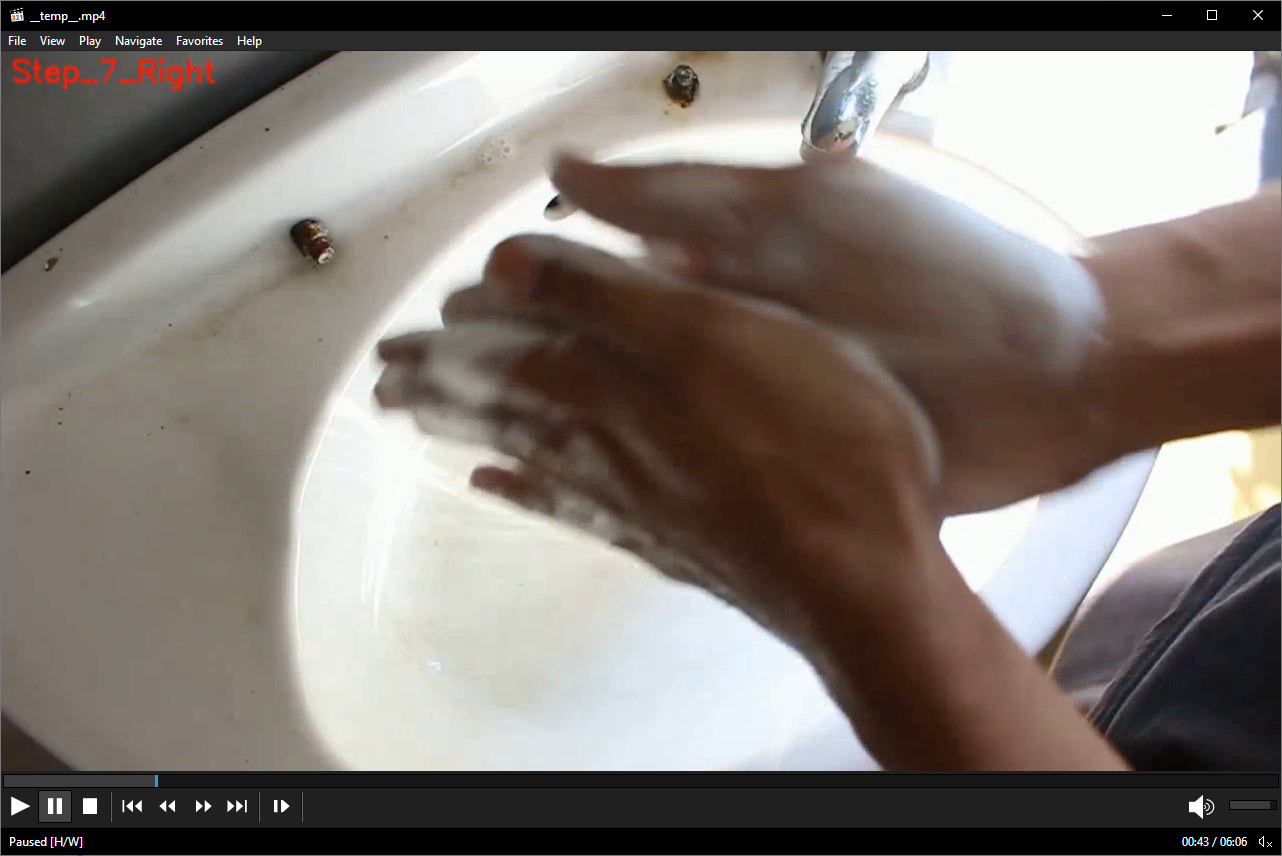
\includegraphics[width=0.6\columnwidth]{gambar/sudutsalah1.png}
	\caption{Pengujian Berdasarkan Sudut (Salah)}
	\label{fig:sudutsalah1}
\end{figure}

Untuk menghindari copyright dan penggunaan yang tidak diinginkan, hasil pengujian selengkapnya dapat disaksikan saksikan pada \textit{Private Link} Berikut :
\begin{center}
	https://youtu.be/q5289IyXDl4
\end{center}

Dari Pengujian yang dilakukan, terlihat bahwa ketika sudut pengambilan video miring maka akan membuat tangan terlihat miring yang mana ini menyebabkan klasifikasi tidak akurat di berberapa titik

\subsection{Pengujian berdasarkan Setup Pengambilan Citra Video}
\label{subsec:ujisetup}

Sample hasi pengujian berdasarkan setup pengambilan citra dapat dilihat pada gambar \ref{fig:setupbenar1} dan \ref{fig:setupsalah1}

\begin{figure}[!ht]
	\centering
	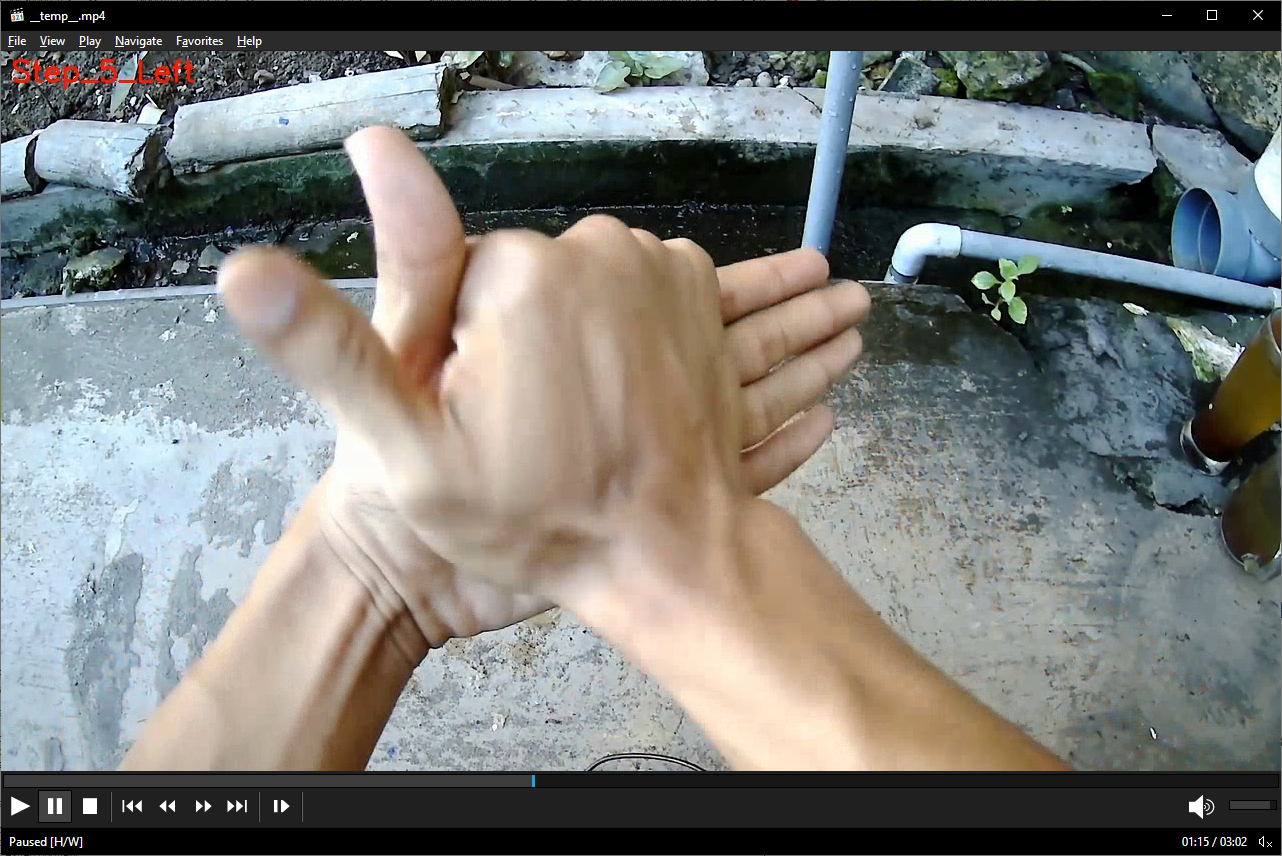
\includegraphics[width=0.6\columnwidth]{gambar/setupbenar1.png}
	\caption{Pengujian Berdasarkan Sudut (Benar)}
	\label{fig:setupbenar1}
\end{figure}
\begin{figure}[!ht]
	\centering
	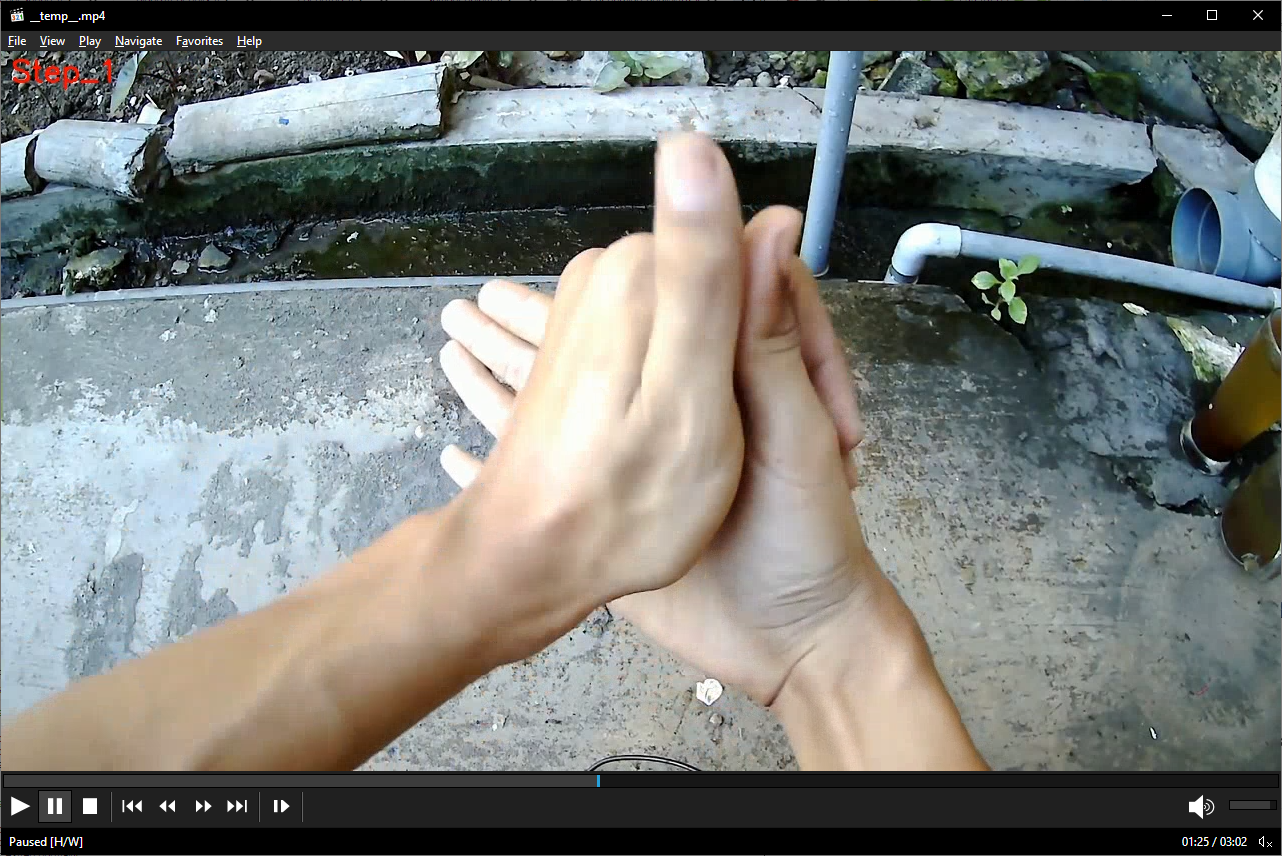
\includegraphics[width=0.6\columnwidth]{gambar/setupsalah1.png}
	\caption{Pengujian Berdasarkan Sudut (Salah)}
	\label{fig:setupsalah1}
\end{figure}

Untuk menghindari copyright dan penggunaan yang tidak diinginkan, hasil pengujian selengkapnya dapat disaksikan saksikan pada \textit{Private Link} Berikut :
\begin{center}
	https://youtu.be/RTlxJlmr5XI
\end{center}

Dari Pengujian yang dilakukan, terlihat bahwa ketika setup video yang digunakan berbeda maka akan menyebabkan klasifikasi tidak akurat di berberapa titik, khususnya ketika ada bagian tangan yang yang menjadi tidak terlihat